% This is "sig-alternate.tex" V2.1 April 2013
% This file should be compiled with V2.5 of "sig-alternate.cls" May 2012
%
% This example file demonstrates the use of the 'sig-alternate.cls'
% V2.5 LaTeX2e document class file. It is for those submitting
% articles to ACM Conference Proceedings WHO DO NOT WISH TO
% STRICTLY ADHERE TO THE SIGS (PUBS-BOARD-ENDORSED) STYLE.
% The 'sig-alternate.cls' file will produce a similar-looking,
% albeit, 'tighter' paper resulting in, invariably, fewer pages.
%
% ----------------------------------------------------------------------------------------------------------------
% This .tex file (and associated .cls V2.5) produces:
%       1) The Permission Statement
%       2) The Conference (location) Info information
%       3) The Copyright Line with ACM data
%       4) NO page numbers
%
% as against the acm_proc_article-sp.cls file which
% DOES NOT produce 1) thru' 3) above.
%
% Using 'sig-alternate.cls' you have control, however, from within
% the source .tex file, over both the CopyrightYear
% (defaulted to 200X) and the ACM Copyright Data
% (defaulted to X-XXXXX-XX-X/XX/XX).
% e.g.
% \CopyrightYear{2007} will cause 2007 to appear in the copyright line.
% \crdata{0-12345-67-8/90/12} will cause 0-12345-67-8/90/12 to appear in the copyright line.
%
% ---------------------------------------------------------------------------------------------------------------
% This .tex source is an example which *does* use
% the .bib file (from which the .bbl file % is produced).
% REMEMBER HOWEVER: After having produced the .bbl file,
% and prior to final submission, you *NEED* to 'insert'
% your .bbl file into your source .tex file so as to provide
% ONE 'self-contained' source file.
%
% ================= IF YOU HAVE QUESTIONS =======================
% Questions regarding the SIGS styles, SIGS policies and
% procedures, Conferences etc. should be sent to
% Adrienne Griscti (griscti@acm.org)
%
% Technical questions _only_ to
% Gerald Murray (murray@hq.acm.org)
% ===============================================================
%
% For tracking purposes - this is V2.0 - May 2012

\documentclass{sig-alternate-05-2015}
\usepackage[utf8]{inputenc}

\begin{document}

% Copyright
\setcopyright{acmcopyright}
%\setcopyright{acmlicensed}
%\setcopyright{rightsretained}
%\setcopyright{usgov}
%\setcopyright{usgovmixed}
%\setcopyright{cagov}
%\setcopyright{cagovmixed}


% DOI
\doi{10.475/123_4}

% ISBN
\isbn{123-4567-24-567/08/06}

%Conference
\conferenceinfo{AsianPLoP 2016}{February 24-26, Taiwan.}

%\acmPrice{\$15.00}

%
% --- Author Metadata here ---
\conferenceinfo{WOODSTOCK}{'97 El Paso, Texas USA}
%\CopyrightYear{2007} % Allows default copyright year (20XX) to be over-ridden - IF NEED BE.
%\crdata{0-12345-67-8/90/01}  % Allows default copyright data (0-89791-88-6/97/05) to be over-ridden - IF NEED BE.
% --- End of Author Metadata ---

\title{A Misuse Pattern for the Web Browser: Modification of traffic}
%\subtitle{[Extended Abstract]
%\titlenote{A full version of this paper is available as
%\textit{Author's Guide to Preparing ACM SIG Proceedings Using
%\LaTeX$2_\epsilon$\ and BibTeX} at


\numberofauthors{3} %  in this sample file, there are a *total*
% of EIGHT authors. SIX appear on the 'first-page' (for formatting
% reasons) and the remaining two appear in the \additionalauthors section.
%

\author{
\alignauthor
Paulina Silva\\
  \affaddr{Departamento de Informática}\\
  \affaddr{Universidad Técnica Federico Santa María}\\
  \affaddr{Valparaíso, Chile}\\
  \email{pasilva@alumnos.inf.utfsm.cl}
% 2nd. author
\alignauthor
Raúl Monge\\
  \affaddr{Departamento de Informática}\\
  \affaddr{Universidad Técnica Federico Santa María}\\
  \affaddr{Valparaíso, Chile}\\
  \email{rmonge@inf.utfsm.cl}
% 3rd. author
\alignauthor 
Eduardo B. Fernandez\\
  \affaddr{Department of Computer \(\&\) Electrical Engineering and Computer Science}\\
  \affaddr{Florida Atlantic University}\\
  \affaddr{Florida, USA}\\
  \email{fernande@fau.edu}
}

\maketitle
\begin{abstract}
Currently, most software development is focused in creating systems connected to the Internet, which allows to add functionality within a system and facilities to their \textit{Stakeholders}. This leads to depend on a \textit{web client}, such as \textit{Web Browser}, which allows access to services, data or operations that the system delivers. However, the Internet influences the attack surface of the system, and unfortunately many stakeholders and developers are not aware of the risks to which they are exposed. The lack of security education among software developers and the scarce and scattered documentation for browsers (and standardization) could become a big problem in large architectural developments that depend on browsers to perform their services. We are studying some security attacks in the web browser by describing them in the form of misuse patterns. A misuse pattern describes how an information misuse is performed from the point of view of the attacker. It defines the environment where the attack is performed, how the attack is performed, countermeasures to stop it, and how to find forensic information to trace the attack once it happens. We are building a catalog of misuse patterns and we present here one we call Modification of traffic in the Web Browser. A catalog of misuse patterns will help designers to evaluate their designs for possible threats.
\end{abstract}


%
% The code below should be generated by the tool at
% http://dl.acm.org/ccs.cfm
% Please copy and paste the code instead of the example below. 
%
\begin{CCSXML}
<ccs2012>
 <concept>
  <concept_id>10010520.10010553.10010562</concept_id>
  <concept_desc>Computer systems organization~Embedded systems</concept_desc>
  <concept_significance>500</concept_significance>
 </concept>
 <concept>
  <concept_id>10010520.10010575.10010755</concept_id>
  <concept_desc>Computer systems organization~Redundancy</concept_desc>
  <concept_significance>300</concept_significance>
 </concept>
 <concept>
  <concept_id>10010520.10010553.10010554</concept_id>
  <concept_desc>Computer systems organization~Robotics</concept_desc>
  <concept_significance>100</concept_significance>
 </concept>
 <concept>
  <concept_id>10003033.10003083.10003095</concept_id>
  <concept_desc>Networks~Network reliability</concept_desc>
  <concept_significance>100</concept_significance>
 </concept>
</ccs2012>  
\end{CCSXML}

\ccsdesc[500]{Computer systems organization~Embedded systems}
\ccsdesc[300]{Computer systems organization~Redundancy}
\ccsdesc{Computer systems organization~Robotics}
\ccsdesc[100]{Networks~Network reliability}




\keywords{Browser, Web Client, Misuse Pattern, Security, Man-in-the-Browser}

\section{Introduction}
%hablar sobre ataques de ingeniería social
The current scenario of attacks in the browser has changed considerably, if compared to those browsers in the 90s. Every day Browsers are more robust and difficult to exploit; therefore, the same attack types, such as drive-by downloads or code-based execution that could subvert a system, are less common every time. A new form of attack has emerged and is fairly easy to achieve, because it is based on deceiving the user to perform what the attacker wants. Once the user is tricked, the attacker can achieve total control over the browser or the host, without having to crack the system \cite{Rajab2013,Labs2013} that hosts the browser. The development of critical systems that interact daily with different users on the network should focus on these attacks because they threaten the confidentiality, integrity and availability of the user's data (personal) as well as the Stakeholders involved.

The new type of attacks described above are called ``social engineering attacks", in \cite{socEngineeering} they are defined as: The act of manipulating someone to perform actions that are not part of the best interests of the victim (person, organization, stakeholder, etc). An attack of this kind can take many forms, there is the possibility of a physical or digital encounter with the victim. Based on social engineering, this attack is one that takes advantage of human behavior and trust of the victim. In the context of web browser, the deceived user is the first and last line of defense against such attacks, the abuse of trust of the user may open the doors of the browser's host, causing damage to both the user and the external systems with which it interacts.

According to studies \cite{browSecPhish,Labs2013,rowSecSEMBlock}, the browser is the first line of defense against multiple Web threats. However, this is affected by the lack of education of users who use browsers and the constant evolution of threats \cite{browSecPhish}. This is why many browser manufacturers have created defense mechanisms such as \cite{Drake2011} that act when the user requests a page, using black or white list, reputation systems \cite{Rajab2013} with warning alerts, among others, so the user can at least avoid the page or choose to enter the malicious site anyway (but no granting access to the page without knowing of the threat).


\section{Misuse Pattern: Modification of traffic in the Web Browser}
We present a misuse pattern that describes a threat found in the Browser Infrastructure we have obtained in a previous work. This threat happens when an attacker is able to compromise the response received from the Provider contacted. An attacker could try to replace some parameters from the response received, delivering a different content from the original to the Browser User (BU).

\subsection*{Intent}
An attacker could modify or give something different than expected when the web Browser User receives the response from the Server or Provider to the Host; by doing so, the browser could interpret the information in a different way than if it had received the original traffic.

\subsection*{Context}
A web browser fetches resources from a Provider to satisfy the access of a Browser User. A Provider has resources in the form of web pages or other web services. The Provider is generally a Web App or Web server, that allows input and output of data to other applications, and usually they are built using HTML, Javascript and CCS. If a server wants to deliver a service, and others want to connect to it, all communication will be done with the HTTP protocol. A Provider, depending on the type, can receive many requests for resources from various host. Depending on the type of request, they may or may not be allowed. For those allowed, the Provider generates a response to the Host, which may come back (or not) to the Browser Client that generated the request.

\subsection*{Problem}
How could an attacker fool the Browser User and Host, by modifying traffic between the entities involved in communication? It is possible that an attacker is hidden in the middle of the communication between the Host and the Provider, resulting in modified content that may affect the Web Content Renderer or the Browser Client. This, in turn, could bring different results, like stealing private information of the Browser User that the Browser Client uses to customize the navigation, such as the authentication token of a Providers. Depending on the type of attacker, it is possible that it may even affect the host where the browser is, leaving the attacker the possibility of performing malicious acts with the host resources.

The attack could take advantage of the following vulnerabilities:
\begin{itemize}
  \item The \textbf{origin} that defines the Same Origin Policy (SOP) which the browser complies, differs in every type of web browser \cite{W3C-SOP,Reis2009, Jackson2008, Crowley2010, Paola2006}.
  \item The \textbf{origin} is not enough as an isolation mechanism between the different resources (web pages, scripts, css and others) \cite{Silic2010, Barth2009, Yason, Liu2012}.
  \item Anyone can create a software component like an extension or plugin for some type of web browser and pass it off as something harmless, consequently a user will not notice the threat and will install it. This could lead to a very known attack named Man-in-the-Browser \cite{Dougan2012,Utakrit2009,Liu2012,Barth2010}. Also, an installed malware (if the user with the required privileges was fooled to make the installation) could affect not only the traffic but also the logs of the systems, so it can erase its trace from the system.
  \item It is possible to affect the Browser Client, and in consequence the Host, without having to find a vulnerability in the system or browser. With social engineering methods it is possible to trick the user, because the Browser User is the weakest link in the system.
  \item The architecture to extend the browser functionality through extensions, plugins and other, depends on the manufacturer, and probably it has a large attack surface.
\end{itemize}

The attack can be facilitated by:
\begin{itemize}
  \item There are many tools for social engineering attacks, that tricks the Browser User into accepting the installation of extensions or malicious plugins more easily.
  \item Any script can be used to exploit the interpreter of the web browser. Often it is also possible to use the same scripting language elements to pass through certain safety barriers provided by the SOP because the language is based on prototypes (ECMAscript).
  \item Manufacturers of browsers still do not have many defense mechanisms that allow an effective identification of malicious resources.
  \item Encryption methods can do nothing against an attack that modifies the traffic before sending or after receiving the message.
\end{itemize}
\subsection*{Solution}
Modifying the traffic in the Web Browser gives attackers the ability to listen, modify and record private information between the Browser User that uses the Host and the Provider that gives the service.

The attacker can safely modify the content of the packets intercepted while acting as a ``Man-in-the-Midddle", but at a different level of abstraction. As the study \cite{Dougan2012} discusses, this approach would usually be commenced with a phishing attack to trick the user into bridging the gap.

This attack compromises the integrity and confidentiallity even if the browser is communicating with a Provider through a secure channel. This is a consequence of the Browser User letting a social engineering attack do its job, by surfing every website without distrust. A single e-mail wishing for the user to click in a URL address could lead into installing a binary, extension or script in the Host.

After a social engineering attack is successful the attacker can take its time, because whatever is installed in the Host, the attacker has installed it with the user's permission, so the social engineering attack is done. Therefore every action done in the Host or Browser Client, will be identified by the Host as an action done by the Browser User, a user of the Host.


\subsection*{Structure}
The structure of the solution used is the same as in our previous work (Browser Infrastructure Pattern). The Attacker class is any entity that could undertake a risky action against the integrity and confidentiality of the browser, the user, Host and Provider (Figure \ref{fig:BIMisuse}). The attacker is able to intercept both the response sent to the Browser Client from the Provider using the Host as a receiver or by having the browser make changes to the input before the messages goes to the Provider, using scripts or other resources.  

\begin{figure*}[h!t]
  \centering
  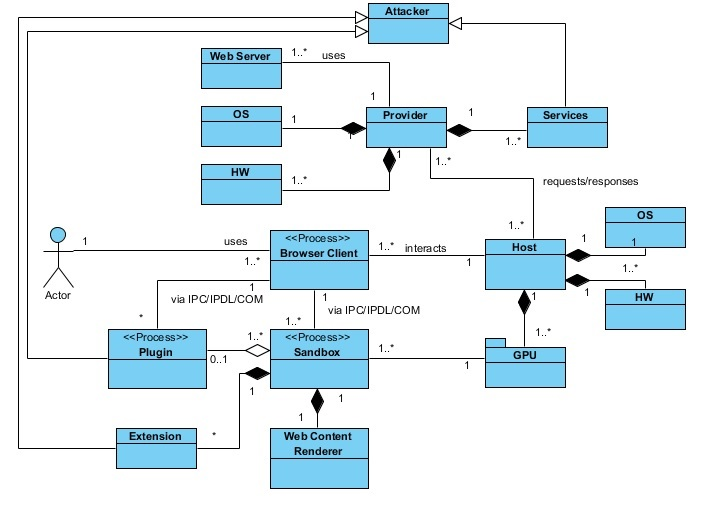
\includegraphics[scale=0.85]{figures/patronMisuse_v6.jpg}
  \caption{Class Diagram for the Misuse Pattern.}
  \label{fig:BIMisuse}
\end{figure*}

\subsection*{Dynamics}
In Figure \ref{fig:SeqMisuse} a series of required steps is shown, for one of the many misuses that can be made for the use case \textbf{Make Request}. The attacker is located between the Browser Client and the Host, intercepting the original request or response and modifying the traffic to its taste; usually an attack basd on this misuse is called Man-in-the-Browser (MITB) \cite{Liu2012, Barth2010, Utakrit2009, Dougan2012}. This could also happen when the Browser User has allowed the installation of plugins, extensions or external programs in the Host and Browser Client.

\begin{figure*}[h!t]
  \centering
  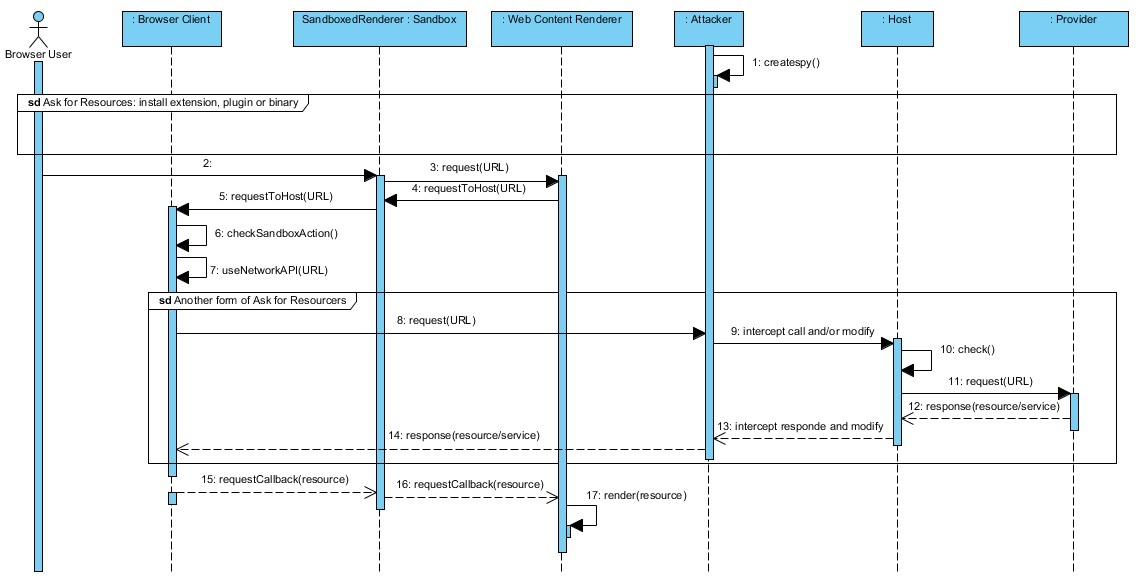
\includegraphics[scale=0.61]{figures/MakeRequestMisuse.jpg}
  \caption{Sequence Diagram for the misuse: Modification of traffic in the Web Browser.}
  \label{fig:SeqMisuse}
\end{figure*}

  
  \subsubsection*{Summary} The attacker instercepts the traffic between the Host and Browser Client.
  \subsubsection*{Actor} Attacker
  \subsubsection*{Precondition} For the attack to go unnoticed, the Browser User must have been tricked by a social engineering attack or the attacker must have directly installed a malicious component or process before in the Host.

  \subsubsection*{Description}
      \begin{enumerate}
        \item An attacker uses a social engineering technique or vulnerability in the system, to create an entity between the Browser Client and Provider and their communication channel, normally a Plugin, binary or Extension.
        \item A Browser User wants to request a resource from a URL, so the first steps are similar to \textbf{Make Request}.
        \item At the time the Browser Client makes a system call to send the message to the Provider, a plugin, an extension or a program in the Host will intercept the message before the system call is done, as the Browser Client has been tapped to perform that action.
        \item The attacker then receives all traffic from the Browser Client, which could be modified or listened.
        \item Finally the victim is compromised.
      \end{enumerate}
  \subsubsection*{Postconditions} The victim will be fully compromised and it probably will not be possible to detect the modification of a message, it is also possible that the log of the Host will be compromised.
  \subsubsection*{Known Uses} The browser is a software that has different implementations, so the number of attack vectors are significant. Some of these are:
      \begin{itemize}
        \item An extension based on the Google Chrome architecture or the Firefox WebExtension API could intercept the data before it reaches the Browser Client or Host \cite{Paola2006}. It could also be possible that a vulnerability in the extension or plugin is used by an attacker and takes advantage of its functionality to attack \cite{Liu2012,Barth2010}. Since the plugin, extension or process are elements the Host trust, it is possible that the attack is undetectable and the encryption methods do not serve as a mitigation measure.
        \item This type of attack can be used as base for more advanced attacks. For example, the browser could have \textit{cross-origin javascript capability leak} vulnerabilities, when different security models such as the one used by Javascript and the DOM interfere with each other. As a consequence, a \textit{cross-origin} request can perform even when the SOP was supposed to stop such attack \cite{Barth2009}.
        \item If neither an extension or plugin is used, a troyan (a downloaded and executed binary) can be another way to get the Host and all the system compromised.
      \end{itemize}


\subsection*{Consequences}
  The misuse has the following consequences for the attacker:
  \begin{itemize}
    \item Objectives: they may be different, we highlight vandalism, impersonate another person or monetary gain. While the attacker may be between the host and the traffic that is sent to the Provider, confidentiality and integrity of the data is completely lost. User privacy can no longer be assured.
    \item Silent: Since the attacker has managed to come between the system calls, that are made to the host, to send data to the Provider, the Host will not recognize or log the anomaly. Calls made to Host are perfectly legal and nothing out of the ordinary, so it will not be seen as something suspicious.
    \item The attacker could perform actions that affect the integrity of the Host.
  \end{itemize}
  Possible sources of error:
  \begin{itemize}
    \item If the Browser User is able to avoid or ignore the social engineering attack carried out at the beginning, this misuse can be subverted. Also, this should consider that the user does not encounter pages with malicious content, which may affect other parts of a browser, but that would cause the same effect as the misuse presented here.
  \end{itemize}

\subsection*{Countermeasures} 
  To prevent this kind of misuse we recommend taking the following preventive measures:
  \begin{itemize}
    \item Reputation services such as SmartScreen \cite{Colvin2010} from Internet Explorer and Download Application \cite{Rajab2013} from Google Chrome, can help to identify pages, web content or resources that could contain malware when is installed as plugins, entensiones or process in the Host of the User Browser.
    \item Providing education about the dangers while surfing the Internet and clarifying the users that they are the last line of defense against such attacks.
    \item Whitelist and Blacklist are installed in the browser as a preventive measure. They help avoid malicious pages or known malware while the user is browsing, they also are updated in a hourly-basis.
    \item Browsers like Google Chrome and Internet Explorer offer Sandboxing. This defense mechanism limits the actions of the attacker, which may affect the integrity of the system.
  \end{itemize}

\subsection*{Forense Evidence}
  Where is it possible to find evidence? Depending on what is desired by the attacker, actions may differ. However the internal log of the browser could help in the audit of the system. This works until an attacker finds a vulnerability in the Sandbox or other component of the browser, in which case he can completely erase its tracks. Also, malware detection such as antivirus systems could help identifying tracks of misuses.

\subsection*{Related Patterns}
  \begin{itemize}
    \item The Browser Infrastructure pattern made in a previous work.
    \item The above pattern, has a class called Browser Client that acts as a Reference Monitor \cite{fernandez2001pattern}.
  \end{itemize}


\section{Conclusions and future work}
%A Web browser appears to be a medium complexity software for users and developers without security experience, but unfortunately this piece of software allows a variaty of attack vectors, to the user using it as well the system with which interacts. Therefore it is important to understand its structure and how it interacts with internal or/and external Stakeholders.

%It is expected that in the future most \textit{Web Browser} will take the form of a Modular Architecture. Therefore, it is important that developers know the internal processes of \textit {browser} when developing a system that will interact with it. The Reference Architecture prepresented here, it is aimed at providing the basic knowledge of the components and interactions between \textit{Web Browser} and external Provider for resources; as well as the threats that exist within it.

%A part of our Reference Architecture has been built through the abstraction of found documentation, through the Browser Infrastructure pattern. We created our first architectural pattern for the infrastructure of \textit{Web Browser}; to help others to understand holistically the components, interactions and relationships of this system. Furthermore it has been possible to characterize the Stakeholders and one of the most important use case. From what we have known, this is the second Reference Architecture for the \textit{Browser} built.

%The proposed work allows a better understanding of this system called Web Browser by using our partially Reference Architecture, this is also helpful to understand existing threats. Furthermore, as it is not subject to specific implementations, it is possible to generalize certain results in other browsers.


We have presented a web browser threat as a form of misuse pattern that systematically describes how one misuse is performed. The aim is to understand and visualize the misuses of the browser that communicates with other systems, mainly to teach developers who have little (or none) security expertise. Through the list of threats done in our previous work, it is possible to detect or infer misuse activities that may appear in one or more misuse cases, which could lead to a violation of the system.

With this misuse pattern we intent to initiated a catalog. This would help to condensate the obtained knowledge using patterns so they can be used as guidelines to communicate relevant concepts, as well as evaluate the existent relationship between the browser and a developed system, to see what kind of interactions they have.

Future work will be related to the creation of a Security Reference Architecture for the \textit{Web Browser} using the same methodology presented here. Other patterns related to Browser Infrastructure pattern will be obtained in order to complete the Reference Architecture we already begun, such as the Web Content Renderer and Browser Kernel pattern. An example of the type of work to be carried out can be seen in \cite{Fernandez2015}. This study was focused on carry out activities to build secure software and evaluate the safety levels of a system already built.

We plan to build more Misuse Patterns for the Browser Infrastructure Pattern, to continue the study of the possible threats in the \textit{Browser}, as a way to educate Developers and Stakeholders. While at the same time these patterns will allow the construction of the Security Reference Architecture. In the same line, in addition to finding potential threats existing in the system, we need to find countermeasures or security defenses to prevent or foresee such threats through security patterns on the reference architecture built. This is possible to perform under the same exercise already conducted in this work, looking for threats at each action for each use case of the Browser.

\bibliography{refTodas}  
\bibliographystyle{IEEEtran}


\end{document}
